%---------------------------------------------------------------------------------------------------
\chapter{Datasets}
\label{chap:datasets}
%---------------------------------------------------------------------------------------------------

In this chapter we introduce the datasets used throughout this dissertation, the Bayesian inference methodology as well as the model and catalog selection criteria.


%---------------------------------------------------------------------------------------------------
\section{Type Ia Supernovae}
\label{sec:SNIa}
%---------------------------------------------------------------------------------------------------

%%% intro to SNIa
A \gls{SNIa} is an event that takes place when a white dwarf in a binary system accretes mass from its companion beyond the Chandrasehkar limit. The result is an explosion of considerable and predictable brightness, which is of great use to study the Universe at cosmological scales.

%%% the reasion why we used SNIa
The usage of \gls{SNIa} on this dissertation will be to provide an additional source of data to complement the constrains set by \gls{SS} events. There are two reasons why we are forced to add an additional source of data. The first is because the model which we will study in the \cref{chap:STG-LCDM-bg} features a degeneracy between two of its parameters in the expression for the luminosity distance for \glspl{GW}, requiring an additional source of data to fix one of its parameters. The second reason is to assist in the model selection which will be carried out in \cref{chap:STG-dark-energy}, between the model which is being studied in that chapter and \gls{LCDM}.

%%% marginalization
The relationship between the apparent magnitude and the luminosity distance is given by

\begin{equation}
    \label{eq:m1}
    m = M + 5 \log{( d_L(z) )} + 25 \,,
\end{equation}
where $M$ is the bolometric magnitude.

Based on \cite{Goliath2001}, we start by taking a standard $\chi^2$ of the form

\begin{equation}
    \chi^2 = \sum_{i=1}^N \left[ \frac{m^\text{(obs)}(z_i) - m(z_i)}{\sigma(z_i)} \right]^2 \,,
\end{equation}
where $m^\text{(obs)}$ is the observed apparent magnitude, $m$ is the theoretical prediction for the apparent magnitude, $N$ the total number of \gls{SNIa} events and finally $z_i$ and $\sigma(z_i)$ are both the redshift and the corresponding error for the $i$-th event.

\Cref{eq:m1} can then be rewritten as

\begin{equation}
    \label{eq:m}
    m = \mathcal{M} + 5 \log{( D_L(z) )} \,,
\end{equation}
where

\begin{equation}
    D_L(z) \equiv \frac{H_0}{c} d_L(z) = (1+z) \int_0^z \frac{1}{E(z)} dz \,,
\end{equation}
is referred to as the $H_0$ independent luminosity distance and $\mathcal{M}$ is defined as

\begin{equation}
    \mathcal{M} \equiv 25 + M + 5 \log{\left( \frac{c}{H_0} \right)} \,.
\end{equation}
We can see that the parameter $M$ is degenerate with $H_0$, we cannot fit either of these parameters separately. Since $\mathcal{M}$ is a nuisance parameter we marginalize it out of the likelihood.

By inserting the apparent magnitude written as presented in \cref{eq:m} in the expression for the $\chi^2$ we obtain that

\begin{equation}
    \chi^2 = \sum_{i=1}^N \left[
    \frac{\Delta^2(z_i)}{\sigma^2(z_i)} -
    2\frac{\Delta(z_i) \mathcal{M}}{\sigma^2(z_i)} +
    \frac{\mathcal{M}^2}{\sigma^2(z_i)}
    \right] \,,
\end{equation}
where we have defined $\Delta(z)$ to be given by

\begin{equation}
    \Delta(z) \equiv m^\text{(obs)} - 5 \log{D_L(z)} \,.
\end{equation}
which can be further simplified to

\begin{equation}
    \label{eq:chi2-no-marginalization}
    \chi^2 = A - 2B\mathcal{M} + \mathcal{M}^2 C \,,
\end{equation}
where $A$, $B$ and $C$ are defined as

\begin{gather}
    A \equiv \sum_{i = 1}^N \frac{\Delta^2(z_i)}{\sigma^2(z_i)} \,, \hspace{1cm}
    B \equiv \sum_{i = 1}^N \frac{\Delta(z_i)}{\sigma^2(z_i)} \,, \hspace{1cm}
    C \equiv \sum_{i = 1}^N \frac{1}{\sigma^2(z_i)} \,.
\end{gather}

We now take the value of $\chi^2$, obtained in \cref{eq:chi2-no-marginalization}, and considering a Gaussian likelihood we marginalize all contributions coming from the term $\mathcal{M}$. Mathematically this is given by

\begin{equation}
    \mathcal{L} = \int_{-\infty}^{\infty} e^{-\chi^2/2} d\mathcal{M} \,,
\end{equation}
which after integrating reduces to

\begin{equation}
    \mathcal{L} = \text{\small $\sqrt{\frac{2 \pi}{C}}$ } \, \text{\Large $e^{\frac{1}{2} (-A + B^2/C)}$ } \,.
\end{equation}

Looking at the expression for the likelihood, we note that there is a multiplicative factor which does not depend on the value of the parameters, but only on the value of the sum of the $\sigma_i$. Given that $\sigma_i$ does not depend on the parameters of our model we can safely drop the multiplicative term to the left of the exponential, simplifying the likelihood for the \gls{SNIa} to

\begin{equation}
    \label{eq:likelihoodsnia}
    \mathcal{L} = \text{\Large $e^{\frac{1}{2} (-A + B^2/C)}$ } \,.
\end{equation}

%%% the SNIa sample we are considering
As for the source of the data, we will be considering \gls{SNIa} events from the Pantheon sample, as was presented in \cite{Pantheon} and is available in a public repository at \cite{Pantheon-repo}. For performance reasons, the binned sample was used throughout this dissertation. We verified that this choice of a reduced sample will not affect our results when compared to the complete dataset.


%---------------------------------------------------------------------------------------------------
\section{Standard Sirens}
\label{sec:SS}
%---------------------------------------------------------------------------------------------------

%%% intro to SS
A \gls{SS} event is any astrophysical phenomena that emits radiation both in the \gls{GW} spectrum, which can be used to directly obtain the luminosity distance of the source, and in the \gls{EM} spectrum, allowing us to obtain the redshift where the event took place. The main source for \gls{SS} events are the merger of massive binary systems, something which is bound to happen for every binary system as they are known to be unstable in \gls{GR}, due to the emission of gravitational waves. By making use of these events, it becomes possible to reconstruct the luminosity distance as a function of redshift, without requiring a ladder distance calibration, making these events prime candidates for testing the evolution of the universe at the very large scales.

%%% intro do LIGO-Virgo
It is the aim of this dissertation, we will study two well known gravitational wave observatories: the advanced \gls{LIGO}, introduced in \cite{advLIGO}, which is a set of two second generation ground based gravitational wave observatories, that together with the advanced Virgo, introduced in \cite{advVirgo}, which is also a second generation ground based observatory, provide the most comprehensive catalog of gravitational wave events to date.

%%% intro to LISA
As for future observatories, we will consider the \gls{LISA}, which aims to be the first \gls{GW} observatory in space by placing three satellites in solar orbit. It has been recently proposed in \cite{LISA-proposal}, with a plan to be launched as early as 2030 and a mission lifetime of 4 years, with a possible extension of up to 10 years. According to \cite{Baker2021} this observatory is expected to be able to detect \gls{GW} events, mostly coming from \glspl{MBHB}, with redshifts up to $z \approx 10$. The data obtained will translate into a major leap in the evaluation of theoretical cosmological settings, given that current measurements have only measured \gls{GW} events with a maximum redshift of $z \approx 1$.

%%% intro to the ET
Additionally, we will also study the \gls{ET}, which is a third generation underground gravitational wave observatory with a successful proposal \cite{Maggiore2020}, that is aimed to have its first light in 2035. Its focus will be mostly targeted towards looking for new physics in high energy events, namely, by looking at the merger of \glspl{BNS}, with the expectations of having a glimpse of its internal structure. Although these events will be probed at low redshifts, they also provide valuable cosmological insight.

%%% why we have to generate SS mock catalogs and how
So far only one \gls{SS} event has been detected so far, named GW170817 \cite{GW170817}, and the possible detection of an \gls{EM} counterpart of GW109521 \cite{GW190521} has been suggested in \cite{GW190521-EM}. Although they were remarkable achievements, with the first event being able to put very tight bounds on the speed of propagation of \glspl{GW}, neither of them is able to put meaningful constrains on either of our models. As such, we choose to create \gls{SS} mock catalogs, which will allow us instead to forecast the constrains set on any given cosmological model, for the \gls{LIGO}-Virgo collaboration, \gls{LISA} and \gls{ET}.

The procedure used to generate the \gls{SS} events is generic, and can be summarized by performing the following steps:

\begin{enumerate}
    \item Obtain a redshift for the event, $z_*$, by sampling the event probability distribution function;
    \item Generate the luminosity distance for the obtained redshift, $d_L(z_*)$, using a fiducial cosmological model.
    \item Compute the error for the obtained redshift for the corresponding observatory, $\sigma_\text{tot}(z_*)$, and consider it to be the $1 \sigma$ region for the luminosity distance;
    \item Consider the observed value of the luminosity distance, $d_L^{(\text{obs})}(z_*)$, to be a sample from a Gaussian distribution with mean in $d_L(z_*)$ and with standard deviation equal to $\sigma_\text{tot}(z_*)$;
    \item Repeat this procedure until we achieve the number of events we expect to observe for each of the observatories considered.
\end{enumerate}

\noindent The last step is performed to obtain a more realistic catalog, such that the most likely value for the observed luminosity distance does not fall consistently on top of the fiducial value. As for the fiducial cosmology, we have decided to consider \gls{LCDM} with fiducial values $h = 0.7$ and $\Omega_m = 0.284$. This latter value corresponds to the best fit for the \gls{SNIa} from the Pantheon sample, such that we avoid tensions between \gls{SS} and \gls{SNIa}.

Following a Bayesian analysis, we take the likelihood for this dataset to be a Gaussian function, which is written as

\begin{equation}
    \label{eq:likelihood-gw}
    \mathcal{L} = \prod_{i=1}^N \frac{1}{\sqrt{2 \pi} \sigma_\text{tot}(z_i)} \exp \left(- \frac{1}{2} \left[ \frac{d_\text{GW}^{\text{(obs)} }(z_i) - d_{\text{GW}}(z_i)}{\sigma_\text{tot}(z_i)} \right]^2 \right) \,,
\end{equation}
where $d^\text{(obs)}_\text{GW}(z)$ is the observed luminosity distance, $d_\text{GW}(z)$ is the theoretical gravitational wave luminosity distance predicted by our model and $N$ is the number of \glspl{SS} events.


%-------------------------------------------------
\subsection{LIGO-Virgo Forecasts}
\label{subsec:ligo-virgo}
%-------------------------------------------------

To obtain the expected probability distribution function of \glspl{SS} events for the \gls{LIGO}-Virgo observatories we take the luminosity distance distribution function found in \cite{Lagos2019}, which is then sampled to obtain the corresponding redshift, using the fiducial cosmology. We then follow the steps 4, 5 and 6 of the mock catalog generation procedure which we have outline before.

Following the steps developed in \cite{Baker2021}, we consider that each \gls{LIGO}-Virgo catalog is composed of $N = 50$ events and the error as a function of redshift is given by
\begin{equation}
    \label{eq:LIGO-error}
    \sigma^2_\text{LIGO-Virgo} = \sigma_{d_L}^2 + \left( \frac{d}{dz}(d_L) \sigma_\text{spect} \right)^2 \,,
\end{equation}
where $\sigma_{d_L}$ is a rough approximation based on the lowest signal-to-noise ratio the \gls{LIGO}-Virgo is expected to measure, given by

\begin{equation}
    \sigma_{d_L} = \frac{5.63 \times 10^{-4}}{\text{Mpc}} d_L^2(z) \,,
\end{equation}
and the second contribution is the propagation to the luminosity distance of the error in the redshift measurement, assumed to be of spectroscopic origin,

\begin{equation}
    \sigma_\text{spect} = 0.005(1+z) \,.
\end{equation}


%-------------------------------------------------
\subsection{LISA}
\label{subsec:LISA}
%-------------------------------------------------

In \cite{Caprini2016} the authors presented the redshift distribution of \glspl{SS} events, which are expected to be visible to LISA. The formation process for \gls{MBHB} events is still not yet fully understood, therefore the authors considered three distinct populations of \glspl{MBHB}: \textit{No Delay}, \textit{Delay} and \textit{Pop III}. For a complete description of each of the populations we refer the reader to \cite{Antonini2015}. The previous redshift distributions were developed for three different mission specifications, throughout this dissertation we have chosen to work with the mission specification L6A2M5N2, since it is the closest to the proposed mission specification presented in \cite{LISA-proposal}.

In order to match the analysis developed in \cite{Speri2021}, we have modified the previous redshift distribution to include no events below $z = 0.1$, justified by the absence of \gls{MBHB} events in this redshift range. For the sake of convenience, we have fitted each of the redshift distribution functions with a beta distribution, which takes the form

\begin{equation}
    \label{eq:beta}
    f(z) = \gamma \left( \frac{z}{9} \right)^{\alpha - 1} \left(1 - \frac{z}{9} \right)^{\beta - 1} \,,
\end{equation}
where the best fit values for each population are shown in \cref{tab:bestfit} and the normalized redshift probability distribution function, as well as the best fit, are represented graphically in \cref{fig:mbhb-dist}.

\begin{figure}[h!]
    \centering
    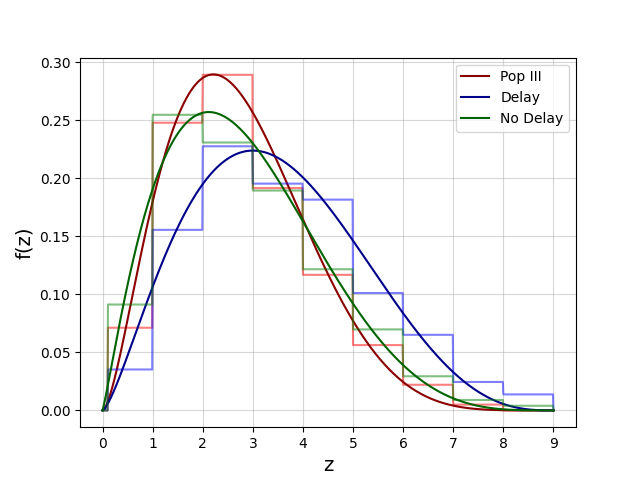
\includegraphics[width=0.65\columnwidth]{figures/MBHB-dist.png}
    \caption[Expected redshift distribution for LISA SS events]
    {Expected normalized redshift distribution for \gls{LISA} \gls{SS}, for the L6A2M5N2 mission specification, for populations \textit{Pop III}, \textit{Delay} and \textit{No Delay}, fitted with \cref{eq:beta}, with the best fit values present in table \ref{tab:bestfit}.}
    \label{fig:mbhb-dist}
\end{figure}

\begin{table}[h!]
    \centering
    \begin{tabular}{|c|c|c|c|}
        \hline
                 & $\alpha$ & $\beta$ & $\gamma$ \\ \hline
        Pop III  & 2.64     & 6.03    & 11.95   \\ \hline
        Delay    & 2.42     & 3.84    & 3.37    \\ \hline
        No Delay & 2.14     & 4.7     & 3.61   \\ \hline
    \end{tabular}
    \caption[Best fit values for a beta distribution applied to the redshift distribution of LISA SS events.]
    {Best fit values of the beta distribution, given by \cref{eq:beta}, for the redshift distribution of the \gls{MBHB} populations \textit{Pop III}, \textit{Delay} and \textit{No Delay}, presented graphically in figure \ref{fig:mbhb-dist}.}
    \label{tab:bestfit}
\end{table}

Based on \cite{Speri2021}, we consider that the total error for the luminosity distance as a function of redshift for \gls{LISA} is given by

\begin{equation}
    \label{eq:LISA-error}
    \begin{aligned}
        \sigma^2_\text{LISA} = \sigma_{\text{delens}}^2 + \sigma_\text{v}^2 + \sigma_{\text{inst}}^2 + \left( \frac{d}{dz} (d_L) \sigma_{\text{photo}} \right)^2 \,,
    \end{aligned}
\end{equation}
where the first term corresponds to the total lensing contribution, which can be decomposed in the multiplication of two factors, given by

\begin{equation}
    \sigma_{\text{delens}} =  F_{\text{delens}} \, \sigma_{\text{lens}} \,,
\end{equation}
where

\begin{equation}
    \sigma_{\text{lens}} = 0.066 \left( \frac{1 - (1+z)^{-0.25}}{0.25} \right)^{1.8} d_L(z) \,,
\end{equation}
is the analytically estimated weak lensing contribution and

\begin{equation}
    F_{\text{delens}} = 1 - \frac{0.3}{\pi/2} \arctan{(z/0.073)} \,,
\end{equation}
is the delensing factor, which includes the possibility of estimating the lensing magnification distribution and partially correct the effect that weak lensing produces on the measurement of the \glspl{GW}.

\noindent The second term considers the error which originates due to the peculiar velocity of the sources, and is estimated to be given by
\begin{equation}
    \sigma_\text{v} = \left[ 1 + \frac{c(1+z)^2}{H(z)d_L(z)} \right] \frac{500 \ \text{km/s}}{c} d_L(z) \,.
\end{equation}

\noindent The third term of the error includes the \gls{LISA} instrumental error on the measurement of the luminosity distance, which can be estimated by

\begin{equation}
    \sigma_{\text{inst}} = 0.05 \left( \frac{d_L^2(z)}{36.6 \text{Gpc}} \right) \,,
\end{equation}
and finally, the last term, includes the redshift error associated with photometric measurements, which is then propagated to the luminosity distance given the fiducial cosmology. We assume this source of error to only take place at redshifts larger than $2$, and takes the form

\begin{equation}
    \sigma_{\text{photo}} = 0.03(1 + z), \text{ if $z > 2$} \,.
\end{equation}

As for the population, according to \cite{Speri2021}, the major difference is expected to come from the number of events detected. As such, we have decided to work with the \textit{No Delay} population, as it seems to provide a middle ground between the other two with respect to the redshift distribution of events.

We then take the most conservative estimate of events expected to detect, for all the \gls{MBHB} populations, which, according to \cite{Tamanini2017}, when using the current hardware specification and a 4 year mission lifetime is $N = 15$ \gls{SS} events.


%-------------------------------------------------
\subsection{Einstein Telescope}
\label{subsec:ET}
%-------------------------------------------------

Following the analysis developed in \cite{Belgacem2018}, the authors expect that the \gls{ET} will observe $N = 10^3$ \gls{SS} events over a three year observation period. The redshift probability distribution function for the \gls{SS} events is given by

\begin{equation}
    f(z) = \frac{4 \pi \mathcal{N} r(z) d_L^2(z)}{H(z)(1+z)^3} \,,
\end{equation}
where $\mathcal{N}$ is a normalization constant used that takes the value required to ensure that $f(z)$ is normalized to unity.

In the previous equation, $z_\text{max}$ is the maximum redshift at which we expect that the \gls{ET} is able to measure an event with a signal-to-noise ratio above 8, which we take to be $z_\text{max} = 2$. The lower cutoff in the integral, $z_\text{min}$, is the lowest redshift which requires a model of the local flow of the emitting source, which we take to be $z_\text{min} = 0.07$.

The function $r(z)$ is called the coalescence rate at redshift $z$, and is given by

\begin{equation}
  r(z) =
    \begin{cases}
      1+2z      & \text{if } 0 \leq z \leq 1 \\
      (15-3z)/4 & \text{if } 1 < z < 5       \\
      0         & \text{if } z > 5           \\
    \end{cases}
\end{equation}
Since we have set an upper and lower cutoff to the observations obtained by the \gls{ET}, the previous function will only be considered inside this redshift range, between $z_\text{min}$ and $z_\text{max}$, instead of between $z = 0$ and $z = 5$.

As for the error, the estimated total error as a function of redshift for the \gls{ET} is considered to be of the form

\begin{equation}
    \label{eq:ET-error}
    \sigma^2_\text{ET} = \sigma^2_\text{inst} + \sigma^2_\text{lens} \,,
\end{equation}
where

\begin{equation}
    \sigma_\text{inst} \approx (0.1449z - 0.0118z^2 + 0.0012z^3) \, d_L(z) \,,
\end{equation}
is the ET instrumental error and

\begin{equation}
    \sigma_\text{lens} \approx 0.05 z \, d_L(z) \,,
\end{equation}
is the error contribution due to lensing. Here we have chosen to neglect the error from the spectroscopic redshift measurements.


%---------------------------------------------------------------------------------------------------
\section{Bayesian Inference Methodology}
\label{sec:sampling-methodology}
%---------------------------------------------------------------------------------------------------

In order to constrain the parameters for each model, we have performed a Bayesian analysis relying on \gls{MCMC} methods. Specifically, we used PyStan \cite{PyStan}, a Python interface to Stan \cite{Stan}, a statistical programming language which implements the No-U-turn sampler, a variant of the Hamiltonian Monte Carlo. The output was then analyzed using GetDist \cite{GetDist}, to perform the corner plot, and ArviZ \cite{arviz}, which is a Python package that allows for an exploratory analysis of Bayesian models, namely by implementing posterior analysis, convergence diagnostics and model selection criteria.

For each combination of model plus dataset, we executed at least 4 independent chains, each of which with at least 2500 samples on the posterior distribution and at least 500 warm-up steps. To ensure that the chains converged, we use the $\hat{R}$ diagnostics, a convergence diagnostics introduced in \cite{Vehtari2021}, where it is claimed to have significant improvements when compared to other convergence diagnostics, namely the widely used Gelman-Rubin test. Roughly speaking, this diagnostics indicates how well the different chains are mixed. In this dissertation we have set an upper bound of $\hat{R} = 1.05$ in all chains, where $\hat{R} = 1$ is the ideal scenario.

The initial values are randomly sampled from a Gaussian distribution with mean around the expected value, which was the value used to generate the mock catalogs, and a standard deviation of roughly 10\% of the corresponding mean for each parameter.

Finally, we consider what we believe to be weakly informative priors, which are given by a Gaussian distribution centered on the expected value and with a standard deviation of approximately two orders of magnitude larger than the previously mentioned value, to ensure a quasi flat prior around the region of interest.


%---------------------------------------------------------------------------------------------------
\section{Model Selection Criteria}
\label{sec:model-selection-criteria}
%---------------------------------------------------------------------------------------------------
% - ref.: https://vasishth.github.io/bayescogsci/book/expected-log-predictive-density-of-a-model.html
% - ref.: FAQ cross-validation - https://mc-stan.org/loo/articles/online-only/faq.html

Throughout this dissertation we will the require to differentiate between two models. To do this we need to evaluate the quality of the posterior predictions for a given model. This can be done by introducing a scoring rule that is referred to as the \gls{elpd} \cite{Gelman2013}, which measures the quality of a model's fit when new data coming from the true data generating process is considered, after constraining the model with a given dataset. Mathematically the \gls{elpd} is given by

\begin{equation}
    \label{eq:elpd}
    \text{elpd} = \sum_{i=1}^N \int p_t(\tilde{y}_i) \ln p(\tilde{y}_i|y) d\tilde{y}_i \,,
\end{equation}
where $N$ is the total number of events, $p_t(\tilde{y}_i)$ is the true distribution that generates the event $\tilde{y}_i$ and $p(\tilde{y}|y)$ is called the posterior predictive distribution which is defined as

\begin{equation}
    p(\tilde{y}|y) = \int p(\tilde{y}_i|\theta) p(\theta|y) d\theta \,,
\end{equation}
where $\theta$ is the vector of the model parameters, $p(\tilde{y}_i|\theta)$ is the probability of observing the event $\tilde{y}_i$ knowing the parameters $\theta$, i.e. the likelihood, and $p(\theta|y)$ is the posterior distribution.

In these very specific circumstances, we know the true distribution $p_t(\tilde{y}_i)$, given that these events are generated and do not correspond to real observations. However, if we are to assume to be oblivious to the data generating process, then we are required to approximate \cref{eq:elpd}.

The method that we will use here is referred to as \gls{LOO-CV}, which consist of fitting our model to $N-1$ events of our dataset, and evaluate how likely is it that this model predicts the left out event. The \gls{elpd} using \gls{LOO-CV} is defined as \cite{Vehtari2015}

\begin{equation}
    \text{elpd}_\text{LOO-CV} = \sum_{i=1}^N \ln p(y_i|y_{-i}) \,,
\end{equation}
where $y_{-i}$ represents the dataset without the $i$-th observation and

\begin{equation}
    p(y_i|y_{-i}) = \int p(y_i|\theta) p(\theta|y_{-i}) d\theta \,,
\end{equation}
gives the probability of predicting the event $y_i$ after constraining the model with the dataset $y_{-i}$.

However, \gls{LOO-CV} methods are very computationally expensive, as one must repeat the full constraining procedure $N$ times, one for each omitted data point. To account for this problem, in \cite{Vehtari2015} the authors present an efficient computation of \gls{LOO-CV}, where a procedure is developed to estimate how the model would look like if constrained using $N - 1$ events, from a single run of \gls{MCMC} with the full sample of $N$ events. This approximation, which is referred to as \gls{PSIS-LOO-CV}, approximates the value of the \gls{elpd} to

\begin{equation}
    \label{eq:elpd_PSIS-LOO-CV}
    \text{elpd}_\text{PSIS-LOO-CV} = \sum_{i=1}^N \ln \left(\frac{\sum_{s=1}^S w_i^s p(y_i|\theta^s)}{\sum_{s=1}^S w_i^s}\right) \,,
\end{equation}
where $\theta^s$ is the $s$-th draw of the posterior distribution $p(\theta|y)$, $S$ is the total number of draws from the previous distribution and $\omega_i^s$ is the weight for the $s$-th draw and for the $i$-th event. The procedure used to compute the weights is detailed in \cite{Vehtari2015}. In order to increase the readability, we will usually refer to the previous quantity simply as \gls{elpd} and state that it was computed using \gls{PSIS-LOO-CV}.

It is clear from the previous expression that a perfect model, i.e. one that would perfectly account for all observations, has an average of the \gls{elpd} equal to zero, since $p(y_i|\theta^s) \approx 1$ for all events $i$, making the argument of the logarithm 1, and the sum over all events equal to 0. This means that, for the same dataset, one model is better than the other if its value of \gls{elpd} is closer to zero. It is also relevant to point out that the  higher the number of observations, the lower the expected value of the average of the \gls{elpd}, since the sum will always include non-positive numbers.

The value for \gls{PSIS-LOO-CV} estimate of the \gls{elpd}, as well as its corresponding standard deviation, is implemented in ArviZ \cite{arviz}, a Python package for Bayesian inference, which was used throughout this dissertation.


%---------------------------------------------------------------------------------------------------
\section{Catalog Selection Criteria}
\label{sec:catalog-selection-criteria}
%---------------------------------------------------------------------------------------------------

To provide statistical confidence that the \glspl{SS} catalogs used throughout this analysis are representative of a wide range of outcomes, we generate several catalogs, for each observatory, and study three representative cases: the best, the median and the worst.

The criteria used to categorize each catalog was based on an how small the multiplication of the 1$\sigma$ region for all parameter is. This value, is formally defined as

\begin{equation}
    \Delta^2_\text{tot} \equiv \prod_{i=1}^N \sigma^2_{\theta_i} \,,
\end{equation}
where $\sigma_{\theta_i}$ is the standard deviation of the parameter $\theta_i$ and $N$ is the total number of parameters. For a given model the value of $\Delta^2_\text{tot}$ dictates how much constraining power a given dataset has, such that the smaller its value, the more certain we are about the values of the parameters.

We refer to the best catalog when we speak of the best possible (generated) outcome, whereas the worst catalog represents the worst possible (generated) outcome and the median catalog has the median constraining power of all of the generated mock catalogs.
